% The China Shock, Re-examined: Beamer version of the Project 1 deck.
% Compile from the output/ folder (e.g. pdflatex, or upload output/ to Overleaf).
\documentclass[11pt]{beamer}
\usepackage[utf8]{inputenc}
\usepackage{booktabs}
\graphicspath{{main/beamer/}{backup/beamer/}}

% UCLA colors, in the style of the course slides (blue title bar, gold title text)
\definecolor{uclablue}{HTML}{2774AE}
\definecolor{ucladarkest}{HTML}{003B5C}
\definecolor{uclagold}{HTML}{FFD100}
\definecolor{uclalight}{HTML}{DAEBFE}
\definecolor{uclagray}{HTML}{EEF1F4}
\definecolor{muted}{HTML}{6B7785}

\usetheme{default}
\setbeamertemplate{navigation symbols}{}
\setbeamercolor{structure}{fg=uclablue}
\setbeamercolor{normal text}{fg=ucladarkest}
\setbeamercolor{frametitle}{bg=uclablue, fg=uclagold}
\setbeamercolor{title}{fg=uclagold}
\setbeamercolor{subtitle}{fg=white}
\setbeamercolor{author}{fg=white}
\setbeamerfont{author}{size=\small}
\setbeamercolor{date}{fg=white}
\setbeamercolor{block title}{bg=uclablue, fg=white}
\setbeamercolor{block body}{bg=uclalight, fg=ucladarkest}
\setbeamercolor{block title alerted}{bg=ucladarkest, fg=uclagold}
\setbeamercolor{block body alerted}{bg=uclagray, fg=ucladarkest}
\setbeamercolor{alerted text}{fg=uclablue}
\setbeamertemplate{itemize items}[circle]
\setbeamertemplate{enumerate items}[circle]
\setbeamertemplate{blocks}[rounded]
\setbeamertemplate{frametitle}{%
  \nointerlineskip
  \begin{beamercolorbox}[wd=\paperwidth, sep=0.45em, leftskip=0.3em, rightskip=0.3em]{frametitle}
    \usebeamerfont{frametitle}\insertframetitle
  \end{beamercolorbox}}
\setbeamertemplate{footline}{%
  \hfill{\tiny\color{muted}\insertframenumber}\hspace{1em}\vspace{0.6em}}

\newcommand{\smallnote}[1]{{\scriptsize\color{muted}\textit{#1}}}
\newcommand{\stat}[2]{%
  \begin{beamercolorbox}[wd=\linewidth, sep=0.6em, rounded=true]{block body}
    {\Large\bfseries\color{uclablue}#1}\par\smallskip
    {\footnotesize #2}
  \end{beamercolorbox}}

\title{The China Shock, Re-examined:\\ What Holds Up?}
\subtitle{Re-testing Autor, Dorn \& Hanson (2013) on U.S.\ local labor markets, 1990--2007}
\author{Alejandro Ba\~{n}ados (UID: 606577549)\\
        Daniela Mendirichaga (UID: 506630528)\\
        Jacob Williams (UID: 006405612)\\
        Niranjana Pasanth (UID: 506787246)}
\date{Econ 424 \textperiodcentered{} Fall 2026}

\begin{document}

% ---------------------------------------------------------------- Title
{
\setbeamercolor{background canvas}{bg=ucladarkest}
\begin{frame}[plain]
  \titlepage
\end{frame}
}

% ---------------------------------------------------------------- 1
\begin{frame}{Only the factory-job losses hold up}
  \small A famous study finds that U.S.\ regions hit harder by Chinese imports lost factory jobs and saw
  more unemployment, more people leaving the workforce, and lower pay. \textbf{We re-ran it three ways.}

  \bigskip
  \begin{columns}[T]
    \column{0.32\textwidth}\stat{1 of 4}{headline effects survives our checks: the loss of factory jobs}
    \column{0.32\textwidth}\stat{$\approx$ half}{the size of that factory-job effect once we control properly}
    \column{0.32\textwidth}\stat{75--80\%}{smaller unemployment and workforce-exit effects; neither is reliable, and the pay effect disappears}
  \end{columns}

  \bigskip
  \begin{alertblock}{Takeaway}
    Treat the factory-job loss as the solid finding. The other effects are unproven.
  \end{alertblock}
\end{frame}

% ---------------------------------------------------------------- 2
\begin{frame}{An influential finding, stress-tested three ways}
  \begin{columns}[T]
    \column{0.46\textwidth}
    \begin{block}{The original claim}
      \footnotesize\textit{Autor, Dorn \& Hanson (2013)}
      \begin{itemize}\footnotesize
        \item Compares 722 U.S.\ local labor markets over 1990--2007
        \item Regions facing more Chinese import competition fared worse on factory jobs,
              unemployment, workforce participation and pay
        \item Widely cited in debates about trade's damage
      \end{itemize}
    \end{block}
    \column{0.5\textwidth}
    \textbf{Our three checks}
    \begin{enumerate}\small
      \item \textbf{1990s only:} does the result hold in the first decade on its own?
      \item \textbf{2000s only:} does it hold in the second decade on its own?
      \item \textbf{Better control:} let factory-heavy regions follow a different path in each decade
    \end{enumerate}
  \end{columns}
  \vfill
  \smallnote{We first reproduced the original results exactly (Backup B2).}
\end{frame}

% ---------------------------------------------------------------- 3
\begin{frame}{Only factory-job losses survive our checks}
  \centering
  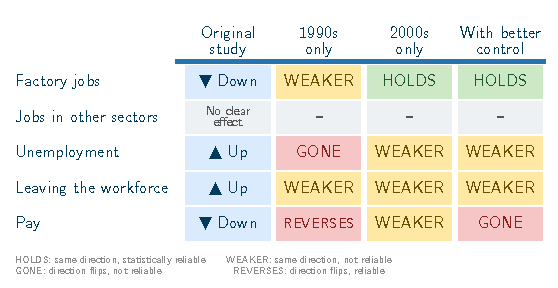
\includegraphics[width=\textwidth, height=0.58\textheight, keepaspectratio]{scorecard}

  \raggedright\small
  \begin{itemize}
    \item \textbf{Factory jobs} survive 2 of 3 checks. \textbf{Unemployment, leaving the workforce and pay} survive none.
    \item In the 1990s alone, the pay effect \textbf{reverses}: exposed regions saw \emph{higher} pay.
  \end{itemize}
\end{frame}

% ---------------------------------------------------------------- 4
\begin{frame}{With a better control, the headline effects shrink by roughly half or more}
  \centering
  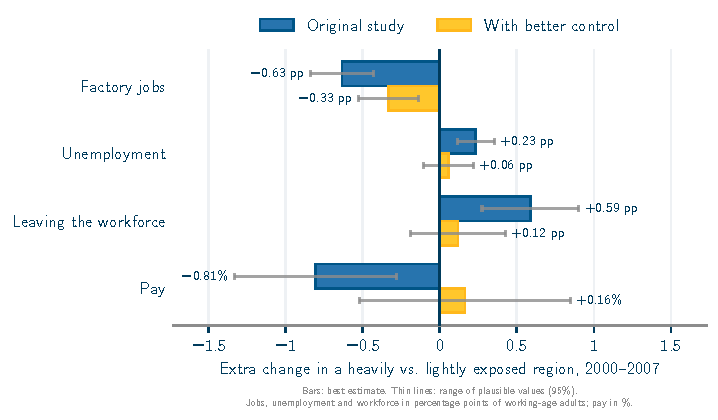
\includegraphics[width=\textwidth, height=0.6\textheight, keepaspectratio]{hero_chart}

  \raggedright\footnotesize
  Heavily vs.\ lightly exposed region (\$1,060 more Chinese imports per worker, 2000--2007):
  factory jobs $-0.63 \rightarrow -0.33$ points (about half, still reliable);
  unemployment $+0.23 \rightarrow +0.06$ (76\% smaller); leaving the workforce $+0.59 \rightarrow +0.12$
  (80\% smaller); pay $-0.8\% \rightarrow +0.2\%$. None but factory jobs is reliable.
\end{frame}

% ---------------------------------------------------------------- 5
\begin{frame}{Factory-heavy regions were declining faster in the 2000s anyway}
  \begin{columns}[T]
    \column{0.55\textwidth}
    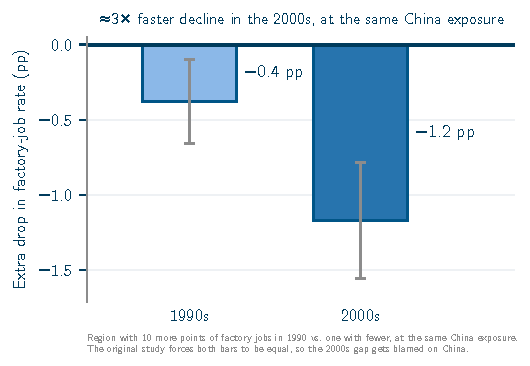
\includegraphics[width=\linewidth]{why_chart}
    \column{0.43\textwidth}
    \begin{itemize}\small
      \item The regions most exposed to China were also the most factory-heavy (correlation 0.54)
      \item \textbf{At the same China exposure}, factory-heavy regions lost factory jobs about
            \textbf{3$\times$ faster in the 2000s} than in the 1990s ($-1.2$ vs.\ $-0.4$ points)
      \item The original study assumes that pattern was the same in both decades, so part of the
            2000s decline gets \textbf{credited to China}
    \end{itemize}
  \end{columns}
\end{frame}

% ---------------------------------------------------------------- 6
\begin{frame}{What this means and what we recommend}
  \begin{columns}[T]
    \column{0.48\textwidth}
    \begin{block}{What we can say}\small
      Chinese import competition shifted jobs away from manufacturing in exposed regions
    \end{block}
    \column{0.48\textwidth}
    \begin{alertblock}{What we can't say}\small
      That it caused lasting, broad increases in unemployment or workforce exit, or lower pay
    \end{alertblock}
  \end{columns}

  \medskip
  \textbf{Recommendations}
  \begin{enumerate}\small
    \item \textbf{Treat the factory-job loss as the solid takeaway,} and the other headline effects as unproven
    \item \textbf{Don't judge a region by ``China-shock devastation'' headlines.} Check current local data instead
    \item \textbf{Before acting on a striking economic finding,} ask whether it survives simple checks like these
  \end{enumerate}
  \vfill
  \smallnote{Data cover 1990--2007. Results compare regions with each other; they are not a forecast.}
\end{frame}

% ---------------------------------------------------------------- Backup
\appendix
{
\setbeamercolor{background canvas}{bg=ucladarkest}
\begin{frame}[plain]
  \vfill
  {\Huge\bfseries\color{white} Backup}\par\medskip
  {\large\color{uclagold} Full results, replication, method checks}
  \vfill
\end{frame}
}

\begin{frame}{B1\quad Full results: all 20 estimates}
  \centering
  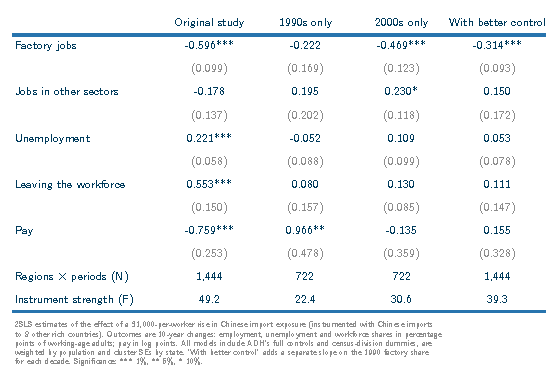
\includegraphics[width=\textwidth, height=0.85\textheight, keepaspectratio]{full_results_table}
\end{frame}

\begin{frame}{B2\quad We reproduce the original study exactly}
  \centering
  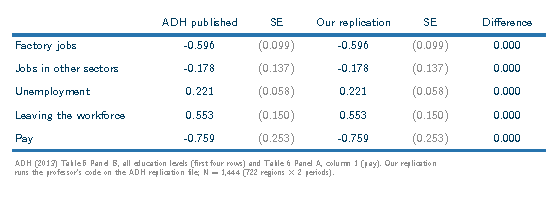
\includegraphics[width=\textwidth]{replication_check}
\end{frame}

\begin{frame}{B3\quad The method's key ingredient is strong in every version}
  \centering
  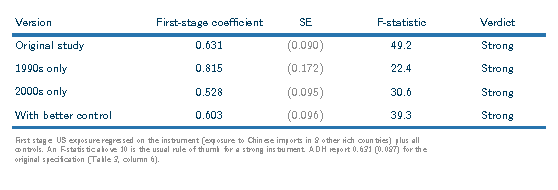
\includegraphics[width=\textwidth]{instrument_strength}

  \raggedright\small
  Strength scores range from 22 to 49. Above 10 is considered strong, so the changes in results are not
  caused by a weak method.
\end{frame}

\begin{frame}{B4\quad Statistically, only the pay effect differs between decades}
  \centering
  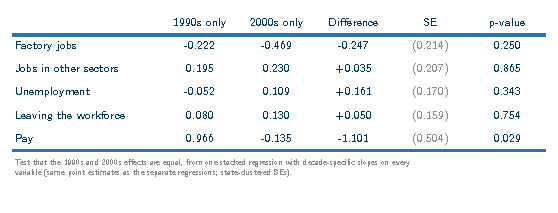
\includegraphics[width=\textwidth]{period_difference_test}

  \raggedright\small
  The single-decade estimates are less precise, so the case rests mainly on the ``better control'' check.
  The decade splits are supporting evidence.
\end{frame}

\begin{frame}{B5\quad All estimates at a glance}
  \centering
  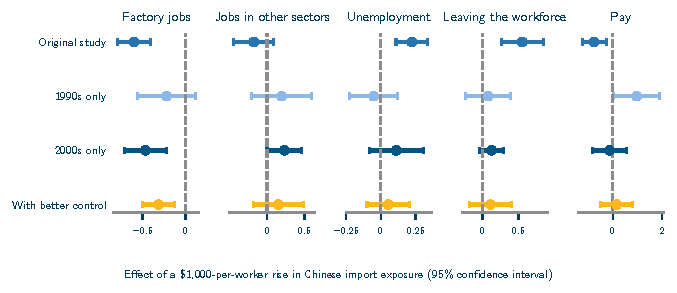
\includegraphics[width=\textwidth, height=0.85\textheight, keepaspectratio]{coefficient_plot}
\end{frame}

\begin{frame}{B6\quad Methods in brief}
  \begin{itemize}\small
    \item \textbf{Data:} replication file from Autor, Dorn \& Hanson (2013): 722 commuting zones $\times$
          2 periods (1990--2000, 2000--2007)
    \item \textbf{Method:} two-stage least squares (2SLS). U.S.\ exposure to Chinese imports is predicted by
          Chinese imports to 8 other high-income countries
    \item \textbf{Setup:} full original controls and census-division dummies, population weights,
          standard errors clustered by state
    \item \textbf{Better control:} a separate effect of the 1990 factory share in each decade
    \item \textbf{Effect sizes:} coefficient $\times$ \$1,060, the gap between the 75th and 25th
          percentile of 2000--2007 exposure
    \item \textbf{Code and results:} \texttt{make\_tables.py} and \texttt{output/backup/}
  \end{itemize}
\end{frame}

\end{document}
